\documentclass[b5paper, 11pt, twoside, onecolumn, openany]{memoir}

%%% PACKAGES
%%%------------------------------------------------------------------------

\usepackage[utf8]{inputenc}
\usepackage[T2A]{fontenc}
\usepackage[greek,english,main=russian]{babel}
\usepackage[final,letterspace=150]{microtype} % Less badboxes
\usepackage{bookmark}
\usepackage{footnotehyper}
\usepackage{multicol}
\usepackage{fancyhdr} % Required by poemscol
\usepackage{poemscol}
\usepackage{geometry}
\usepackage{pifont}
\usepackage{xcolor}

% \usepackage{kpfonts} %Font

\usepackage{amsmath,amssymb,mathtools} % Math

% \usepackage{tikz} % Figures
\usepackage{graphicx} % Include figures

%%% PAGE LAYOUT
%%%------------------------------------------------------------------------

\setlrmarginsandblock{0.11\paperwidth}{*}{1} % Left and right margin
\setulmarginsandblock{0.14\paperwidth}{*}{1} % Upper and lower margin
\checkandfixthelayout

\clubpenalty=10000
\widowpenalty=10000
\raggedbottom

%%% SECTIONAL DIVISIONS
%%%------------------------------------------------------------------------

\maxsecnumdepth{section} % Subsections (and higher) are numbered
\setsecnumdepth{section}

\makeatletter %
\makechapterstyle{standard}{
  \setlength{\beforechapskip}{0.8\baselineskip}
  \setlength{\midchapskip}{0\baselineskip}
  \setlength{\afterchapskip}{0.5\baselineskip}
  \renewcommand{\chapterheadstart}{\vspace*{\beforechapskip}}
  \renewcommand{\chapnamefont}{\centering\normalfont\Large}
  \renewcommand{\printchaptername}{\chapnamefont \@chapapp}
  \renewcommand{\chapternamenum}{\space}
  \renewcommand{\chapnumfont}{\normalfont\Large}
  \renewcommand{\printchapternum}{\chapnumfont \thechapter}
  \renewcommand{\afterchapternum}{\par\nobreak\vskip \midchapskip}
  \renewcommand{\printchapternonum}{\vspace*{\midchapskip}\vspace*{5mm}}
  \renewcommand{\chaptitlefont}{\centering\bfseries\normalsize}
  \renewcommand{\printchaptertitle}[1]{\chaptitlefont ##1}
  \renewcommand{\afterchaptertitle}{\par\nobreak\vskip \afterchapskip}

  % Part titles
  \renewcommand{\beforepartskip}{}
  \renewcommand{\afterpartskip}{\bigskip}

  \renewcommand{\clearforchapter}{}
}
\makeatother

\chapterstyle{standard}

\newcommand{\styledsubsubsection}[2][]{%
  \subsubsection[#1]{\normalsize\mdseries\em #2}}

\newcommand{\addtocspace}[1]{%
  \addtocontents{toc}{\vspace{#1}}}

\newcommand{\hegpart}[2][]{%
  \addtocontents{toc}{\vspace{4mm}%
    {\centering\bfseries\em #1\\\vspace{2mm}}}%
  \part[\small\MakeUppercase{#2}]%
       {\begin{Spacing}{1.6}\small\textsc{\lsstyle\mdseries%
        #1}\nopagebreak\\\normalsize\MakeUppercase{#2}\end{Spacing}}}

\newcommand{\hegchapter}[2][]{%
  \chapter[{\em #1.} #2]{%
    \fontsize{11}{18}\selectfont{\em\mdseries #1}\nopagebreak\\%
    \vspace{1mm}\\%
    \MakeUppercase{#2}%
    \nopagebreak%
    \vspace{2mm}\\}%
    \addtocspace{1mm}%
    \thispagestyle{plain}}

\newcommand{\hegsection}[2][]{%
  \section[#1]{\small\MakeUppercase{#2}}}

\newcommand{\hegremark}[3][]{%
  \subsubsection[#1. #2]{\centering {\lsstyle\mdseries #1}\nopagebreak\\%
  \vspace{1mm}\\%
  \footnotesize #3}}

\setsecheadstyle{\normalfont\bfseries\centering}
\setsubsecheadstyle{\normalfont\normalsize\bfseries\centering}
\setparaheadstyle{\normalfont\normalsize\bfseries}
\setparaindent{0pt}\setafterparaskip{0pt}

\usepackage{indentfirst}
\setlength\parindent{6mm}

%%% FLOATS AND CAPTIONS
%%%------------------------------------------------------------------------

\makeatletter % You do not need to write [htpb] all the time
\renewcommand\fps@figure{htbp}
\renewcommand\fps@table{htbp}
\makeatother

\captiondelim{\space } % A space between caption name and text
\captionnamefont{\small\bfseries} % Font of the caption name
\captiontitlefont{\small\normalfont} % Font of the caption text

\changecaptionwidth % Change the width of the caption
\captionwidth{1\textwidth}

%%% ABSTRACT
%%%------------------------------------------------------------------------

\renewcommand{\abstractnamefont}{\normalfont\small\bfseries} % Abstract title
\setlength{\absleftindent}{0.1\textwidth} % Width of abstract
\setlength{\absrightindent}{\absleftindent}

\tightlists

%%% HEADER AND FOOTER
%%%------------------------------------------------------------------------

\makepagestyle{standard} % Make standard pagestyle

\makeatletter % Define standard pagestyle
\makeevenfoot{standard}{}{}{}
\makeoddfoot{standard}{}{}{}
\makeevenhead{standard}{\bfseries\thepage\normalfont\qquad\small\leftmark}{}{}
\makeoddhead{standard}{}{}{\small\rightmark\qquad\bfseries\thepage}
% \makeheadrule{standard}{\textwidth}{\normalrulethickness}
\makeatother

\makeatletter
\makepsmarks{standard}{
\createmark{chapter}{both}{nonumber}{\@chapapp\ }{ \quad }
\createmark{chapter}{right}{nonumber}{}{ \quad }
\createmark{section}{right}{nonumber}{}{ \quad }
\createmark{subsection}{right}{nonumber}{}{ \quad }
\createplainmark{toc}{both}{\contentsname}
\createplainmark{lof}{both}{\listfigurename}
\createplainmark{lot}{both}{\listtablename}
\createplainmark{bib}{both}{\bibname}
\createplainmark{index}{both}{\indexname}
\createplainmark{glossary}{both}{\glossaryname}
}
\makeatother                               %

\makepagestyle{chap} % Make new chapter pagestyle

\makeatletter
\makeevenfoot{chap}{}{}{} % Define new chapter pagestyle
\makeoddfoot{chap}{}{}{}
\makeevenhead{chap}{}{}{}
\makeoddhead{chap}{}{}{}
% \makeheadrule{chap}{\textwidth}{\normalrulethickness}
\makeatother

\nouppercaseheads
\pagestyle{standard}   % Choosing pagestyle and chapter pagestyle
\aliaspagestyle{chapter}{chap}

%%% END NOTES
%%%------------------------------------------------------------------------
\makepagenote
\continuousnotenums
\notepageref

\let\oldpagenote\pagenote%
  \renewcommand{\pagenote}[1]{%
  {\fontsize{8}{8}\selectfont%
  \:\oldpagenote{#1}}}

\let\oldfootnote\footnote%
  \renewcommand{\footnote}[1]{%
  \,\oldfootnote{~#1}}

\renewcommand{\noteidinnotes}[2]{%
  \hspace{9mm}\textsuperscript{#1}\hspace{1.5mm}}
\renewcommand{\pageinnotes}[1]{%
  К~\hyperref[#1]{стр.~\pageref*{#1}.} ---}

\renewcommand*{\thefootnote}{\ding{93}}

\renewcommand*{\footnoterule}{%
  \kern-3pt%
  \hrule width 0.17\columnwidth
  \kern 2.6pt
  \vspace{1mm}}

\renewcommand*{\notedivision}{}

\renewcommand*{\pagenotesubhead}[3]{}

\renewcommand*{\pagenotesubheadstarred}[3]{}

%%% TEXT
%%%------------------------------------------------------------------------

\renewcommand{\baselinestretch}{0.82}
\setPagenoteSpacing{0.82}
\setFloatSpacing{0.82}

%%% NEW COMMANDS
%%%------------------------------------------------------------------------

\newcommand{\hm}[1]{#1\nobreak\discretionary{}{\hbox{\ensuremath{#1}}}{}}

\maxtocdepth{paragraph} % ToC depth
\settocdepth{paragraph}
\addto\captionsrussian{\renewcommand{\contentsname}{ОГЛАВЛЕНИЕ}}
\setlength{\cftbeforepartskip}{0.5mm}

\AtEndDocument{\addtocontents{toc}{\par}} % Add a \par to the end of the TOC

\usepackage{hyperref}   % Internal hyperlinks
\hypersetup{
  pdfborder={0 0 0},    % No borders around internal hyperlinks
  pdfauthor={ФРА}       % author
}
\usepackage{memhfixc}

\author{Г.~В.~Ф. Гегель}
\title{Наука логики}
\date{}

\renewcommand{\partnumberline}[1]{} % Remove part number in ToC
\renewcommand{\cftpartdotsep}{\cftdotsep} % Part dots in ToC
\renewcommand{\chapternumberline}[1]{} % Remove chapter number in ToC
\renewcommand{\cftchapterdotsep}{\cftdotsep} % Chapter dots in ToC

\renewcommand{\printpartname}{}
\renewcommand{\thepart}{}

\renewcommand{\printchaptername}{}
\renewcommand{\thechapter}{}

\makeatletter
\renewcommand{\@seccntformat}[1]{}
\makeatother

% Remove section numbers in ToC
\let\oldcftsf\cftsectionfont% save definition of \cftsectionfont
\let\oldcftspn\cftsectionafterpnum% and of \cftsectionafterpnum
\renewcommand*{\cftsectionfont}{%
\let\oldnl\numberline% save definition of \numberline
\renewcommand*{\numberline}[1]{}% change it
\oldcftsf} % use original \cftsectionfont
\renewcommand*{\cftsectionafterpnum}{%
\let\numberline\oldnl% % restore orginal \numberline
\oldcftspn} % use original \cftsectionafterpnum

\cftpagenumbersoff{book}
\renewcommand*{\cftbookfont}{\hfil}
\renewcommand*{\cftbookafterpnum}{\hfil}

\begin{document}

\frontmatter
\pagestyle{empty}

{\centering
  {\Large Г.~В.~Ф.~ГЕГЕЛЬ} \\
  \vspace{130pt}
  \textbf{\Huge \textcolor{red}{\fontsize{50pt}{60pt}\selectfont НАУКА ЛОГИКИ}} \\
  \vspace{30pt}
  {\huge Издание в~продолжениях. Выпуск 1} \\
  \vspace{60pt}
  {\Large Том~I. Объективная логика} \\
  \vspace{8pt}
  {\large Книга~I. Учение о~бытии} \\
  \vspace{8pt}
  {\large Глава~I. Бытие} \\
  \vspace{210pt}
  {\tiny ЛАТВИЙСКОЕ ИЗДАТЕЛЬСТВО НАУЧНО-ПОЛИТИЧЕСКОЙ ЛИТЕРАТУРЫ} \\
  \vspace{10pt}
  {\small \textit{РИГА \ \ \ 2025}} \\
\par}

\clearpage

\pagestyle{empty}

\newgeometry{left=15mm,right=15mm,top=25mm,bottom=5mm}

\begin{center}
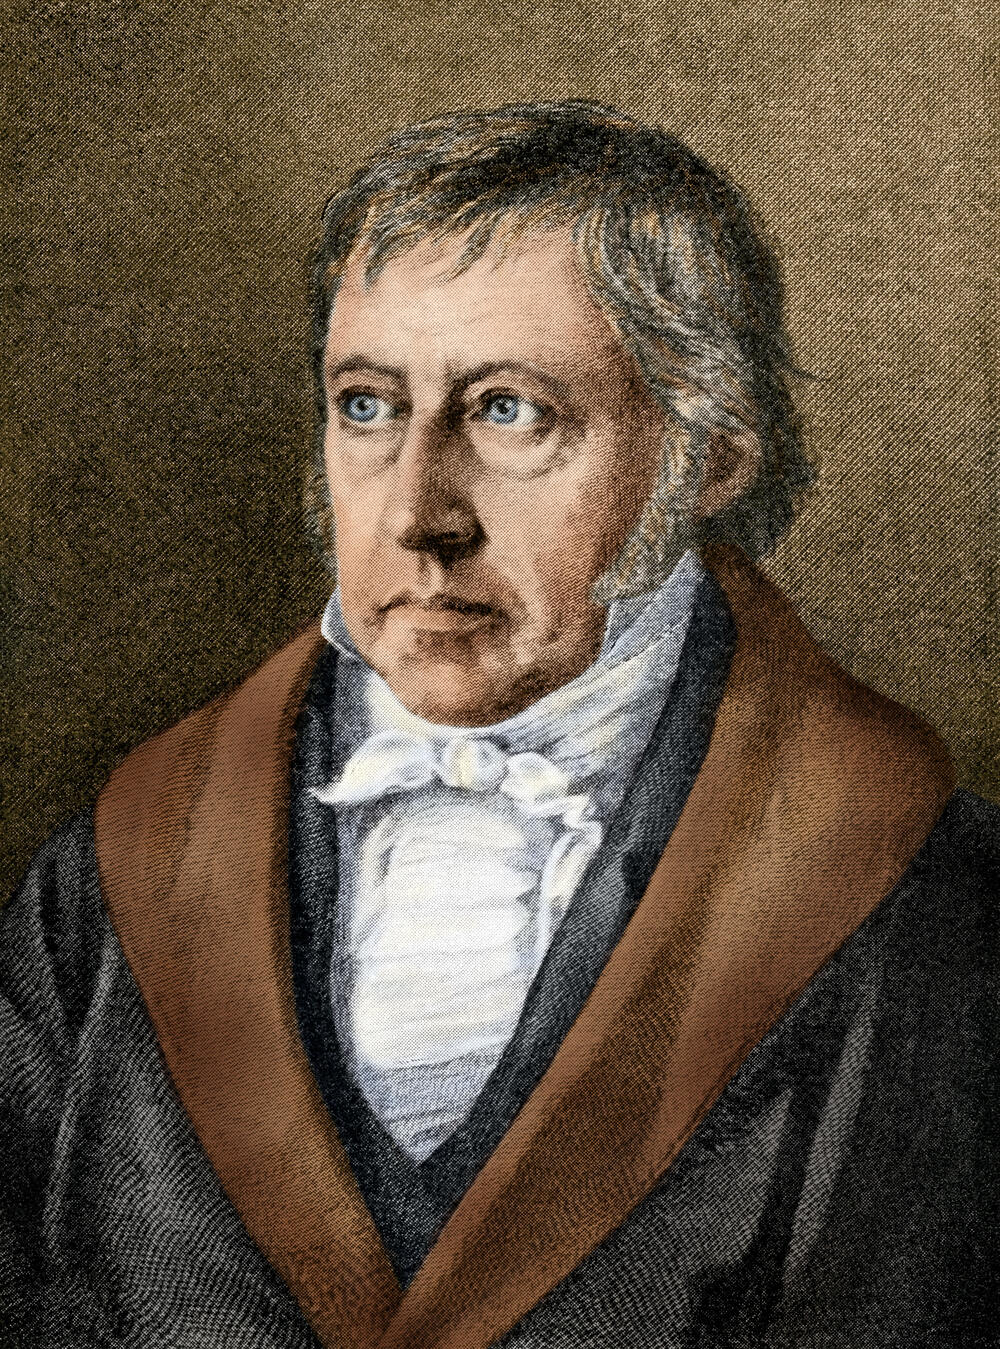
\includegraphics[width=14cm]{hegel-img001.jpg}
\end{center}

\restoregeometry

\mainmatter

\pagestyle{plain}

\addtocontents{toc}{\vspace{7mm}%
  {\centering\lsstyle\normalsize\bfseries Первая книга\\}%
   \vspace{2mm}}

\part[\hspace{38mm}УЧЕНИЕ О~БЫТИИ]%
     {\ \\\vspace{200pt}\Large\mdseries ПЕРВАЯ КНИГА\\\ \\
      \LARGE\bfseries УЧЕНИЕ О~БЫТИИ}
\addtocspace{2mm}

\hegpart[Первый отдел]{Определённость (качество)}

% Первая глава. Бытие.
\clearpage

Бытие есть неопределенное непосредственное. Оно свободно от определенности
по отношению к сущности, равно как еще свободно от всякой определенности,
которую оно может получить внутри самого себя. Это не имеющее рефлексии
бытие есть бытие, как оно есть непосредственно лишь в самом себе.

Так как оно неопределённо, то оно есть бескачественное бытие.
Но~{\em в~себе} ему принадлежит характер неопределённости
лишь в~противоположность к~{\em определённому} или
качественному. Но~бытию~вообще противостоит
{\em определённое} бытие как~таковое, а~благодаря этому
сама его неопределённость составляет его качество. Тем~самым
обнаружится, что {\em первое}~бытие есть определенное~в~себе
и~что, следовательно:

{\em во-вторых}, оно переходит в
{\em наличное бытие}, есть
{\em наличное бытие}, но что последнее как конечное
бытие снимает себя и переходит в бесконечное соотношение бытия с самим
собою,

переходит, {\em в-третьих}, в
{\em для-себя-бытие}.

\chapter[{\em Первая глава} Бытие]{Первая глава. Бытие.}
\section[А. Бытие]{А. Бытие}

{\em Бытие}, {\em чистое бытие} "--- без всякого дальнейшего определения.
В~своей неопределенной непосредственности оно равно лишь
самому себе, и~оно также и~не~неравно по отношению к~иному, не~имеет
никакой разности ни внутри себя, ни по~отношению к~внешнему. Если бы
в~нём было какое-либо определение или
содержание, отличное от~иного определения в~нём~же, или же такое
определение или содержание, которым оно отличается от~некоего иного
бытия, то~такое различие нарушило~бы его чистоту. Бытие есть чистая
неопределенность и~пустота. --- В~нём нечего созерцать, если здесь
может идти речь о~созерцании, или, иначе~говоря, оно есть~только само
это чистое, пустое созерцание.
В~нём столь же мало есть нечто такое, что можно было~бы
мыслить, или, иначе~говоря, оно равным образом есть~лишь это пустое
мышление. Бытие, неопределенное, непосредственное, есть~на~деле
{\em ничто} и~не~более и~не~менее, чем~ничто.

\section[В. Ничто]{В. Ничто}
{\em Ничто}, {\em чистое ничто}; оно
есть простое равенство с~самим собою, совершенная пустота, отсутствие
определений и~содержания; неразличенность в~самом~себе. --- Поскольку
здесь можно говорить о~созерцании или мышлении, следует сказать,
что~считается небезразличным, созерцаем~ли мы, а~также мыслим~ли мы
нечто~или {\em ничто}. Выражение <<созерцать или мыслить ничто>>,
следовательно, что-то означает. Мы проводим различие между этими двумя
случаями; таким образом, ничто {\em есть} (существует)
в нашем созерцании или мышлении; или, вернее, оно~и~есть само~это пустое
мышление и~созерцание; и~оно~есть то~же~самое пустое созерцание или
мышление, что~и чистое бытие. --- Ничто есть, стало быть, то~же~самое
определение или, вернее, то~же~самое отсутствие определений и,~значит,
вообще то~же~самое, что~и чистое {\em бытие}.

\section[С. Становление]{С. Становление}
\subsection[1. Единство бытия и ничто]{1. Единство бытия и ничто}
{\em Чистое бытие и~чистое ничто есть},
{\em следовательно}, {\em одно и~то~же}.
Истина состоит не~в~бытии и~не~в~ничто, а~в~том, что~бытие "---
не~переходит, а "--- перешло в~ничто, и~ничто "---~не~переходит,
а "---~перешло в~бытие. Но равным образом истина заключается
не~в~их неразличенности, а~в~том, что {\em они не одно~и~то~же}, что
{\em они абсолютно различны}, но~столь~же и~нераздельны
и~неотделимы и~что {\em каждое} из~них непосредственно
{\em исчезает в~своей противоположности}. Их истина
есть, следовательно, это {\em движение}
непосредственного исчезновения одного в другом:
{\em становление}; такое~движение, в~котором они оба
различны, но~таким~различием, которое столь~же непосредственно
растворилось.

\subsubsection[Примечание 1. Противоположность бытия и ничто в представлении]
{Примечание 1. Противоположность бытия и ничто в представлении}\pagenote{В квадратных
скобках даются заголовки примечаний, приведенные у Гегеля в оглавлении
«Науки логики», но отсутствующие в самом тексте (см. замечание Ленина по
этому поводу в «Философских тетрадях», Москва 1933, стр. 122).}

{\em Ничто} обыкновенно противополагается [категории]
{\em нечто}; но нечто есть уже некое определенное,
сущее, отличающееся от иного {\em нечто}; таким
образом и ничто, противополагаемое [категории] нечто, есть ничто
какого-либо нечто, некое определенное ничто. Но здесь мы должны брать ничто
в его неопределенной простоте. "--- Если бы кто-нибудь считал более правильным
противополагать бытию {\em небытие} вместо ничто, то мы
не имели бы, что возразить против этого в рассуждении получающегося
результата, ибо в {\em небытии} содержится соотношение
с {\em бытием}; оно есть и то и другое, бытие и его
отрицание, высказанные одним духом, ничто, каково оно в становлении. Но
здесь ближайшим образом идет речь не о форме противоположения,~т.~е.
одновременно и о форме {\em соотношения}, а об
абстрактном, непосредственном отрицании, о ничто, взятом чисто само по
себе, о безотносительном отрицании, "--- что, если угодно, можно было бы
выразить также и простым <<{\em не}>>.

Простую мысль о {\em чистом бытии} как об абсолютном и
как единственную истину высказали впервые {\em элеаты},
преимущественно {\em Парменид}, и последний в
сохранившихся после него фрагментах высказал ее с чистым воодушевлением
мышления, в первый раз постигшего себя в своей абсолютной абстрактности:
{\em лишь бытие есть}, {\em а
небытия вовсе нет}. "--- В восточных системах, главным образом в буддизме,
{\em ничто}, пустота, является, как известно,
абсолютным принципом. "--- Глубокомысленный {\em Гераклит}
выдвинул в противоположность вышеуказанной простой и односторонней
абстракции более высокое, целостное понятие становления и сказал:
{\em бытие столь же мало есть},
{\em как и небытие}, или, выражая эту мысль также и
иначе, говорил: <<все{\em  течет}>>,~т.~е. все есть
{\em становление}. "--- Популярные, в особенности
восточные, изречения, гласящие, что все, что есть, носит зародыш своего
уничтожения в самом своем рождении, а смерть есть, наоборот, вступление в
новую жизнь, выражают в сущности то же самое единение бытия и ничто. Но эти
выражения предполагают субстрат, в котором совершается переход: бытие и
ничто удерживаются вне друг друга во времени, представляются как бы
чередующимися в нем, а не мыслятся в их абстрактности, и поэтому также и не
мыслятся так, чтобы они сами по себе были одним и тем же.

<<Ex nihilo nihil fit>> (ничто не происходит из ничего) "---~есть одно из тех
положений, которым некогда приписывалось в метафизике большое значение. В
этом положении можно либо усматривать лишь бессодержательную тавтологию:
ничто есть ничто; либо, если действительным смыслом этого положения
является высказывание о {\em становлении}, приходится
сказать, что так как из {\em ничего становится}
{\em ничто же}, то на самом деле здесь нет речи о
становлении, ибо ничто здесь так и остается ничем. <<Становление>> означает,
что ничто не остается ничем, а переходит в свое иное, в бытие. "--- Если
позднейшая метафизика, главным образом христианская, отвергла положение,
гласящее, что из ничего ничего не происходит, то она этим утверждала
переход ничто в бытие; как бы синтетически или, иначе сказать, в форме
просто представления она ни брала последнее положение, все же даже в самом
несовершенном соединении имеется точка, в которой бытие и ничто встречаются
и их различие исчезает. "--- Подлинную свою важность положение:
{\em из ничего ничего не происходит},
{\em ничто есть именно ничто}, получает благодаря его
антагонизму к {\em становлению} вообще и,
следовательно, также к сотворению мира из ничего. Те, которые утверждают
положение: ничто есть именно ничто, и даже горячо отстаивают его, не
сознают того, что они тем самым соглашаются с абстрактным
{\em пантеизмом} элеатов и по сути дела также и со
спинозовским пантеизмом. Философское воззрение, которое считает принципом
положение: <<бытие есть только бытие, ничто есть только ничто>>, заслуживает
названия системы тождества; это абстрактное тождество представляет собою
сущность пантеизма.

Если вывод, что бытие и ничто суть одно и то же, взятый сам по себе, кажется
удивительным или парадоксальным, то мы в дальнейшем не должны обращать на
это внимания; скорее приходится удивляться этому удивлению, которое
показывает себя таким новичком в философии и забывает, что в этой науке
встречаются совсем иные определения, чем те, которые имеют место в
обыденном сознании и в так называемом здравом человеческом рассудке,
который как раз не всегда есть здравый, а есть также рассудок, специально
культивированный для абстракций и для веры в них или, вернее, для
суеверного отношения к абстракциям. Было бы нетрудно показать наличие этого
единства бытия и ничто на всяком примере во всякой действительной вещи или
мысли. Относительно {\em бытия} и
{\em ничто} следует сказать то же самое, что мы сказали
выше относительно непосредственности и опосредствования (каковое последнее
заключает в себе некое соотношение {\em друг с другом}
и, значит, {\em отрицание}), а именно, что
{\em нет ничего ни на небе, ни на земле, что не
содержало бы в себе и того и иного, и бытия и ничто}. Так как при этом
начинают говорить о {\em каком-нибудь определенном
нечто и действительном}, то, разумеется, в этом нечто указанные определения
уже больше не наличествуют в той совершенной неистинности, в каковой они
выступают как бытие и ничто, а в некотором дальнейшем определении и
понимаются, например, как {\em положительное} и
{\em отрицательное}; первое есть положенное,
рефлектированное бытие, а последнее есть положенное, рефлектированное
ничто; но положительное и отрицательное содержат в себе как свою
абстрактную основу первое "---~бытие, а второе "---~ничто. "--- Так, например, в
самом боге качество, {\em деятельность},
{\em творение}, {\em могущество}
и~т.~д. содержат в себе по существу определение отрицательного, "--- они суть
продуцирование некоторого {\em иного}. Но
эмпирическое пояснение указанного положения примерами было бы здесь
совершенно излишне. Так как мы теперь знаем раз навсегда, что это единство
бытия и ничто лежит в основании в качестве первой истины и составляет
стихию всего последующего, то помимо самого становления все дальнейшие
логические определения: наличное бытие, качество, да и вообще все понятия
философии служат примерами этого единства. А так называющий себя
обыкновенный или здравый человеческий рассудок, поскольку он отвергает
нераздельность бытия и ничто, мы можем пригласить сделать попытку отыскать
пример, в котором мы могли бы найти одно отделенным от другого (нечто от
границы, предела, или бесконечное, бог, как мы только что упомянули, от
деятельности). Только пустые, сочиненные мыслью вещи (Gedankendinge)
"---~бытие и ничто "---~только сами они и суть такого рода раздельные, и их-то
вышеуказанный рассудок предпочитает истине, нераздельности, которую мы
повсюду имеем перед собой.

Нашим намерением не может быть всесторонне предупредить сбивчивые
возражения, путаные соображения, выдвигаемые обыденным сознанием, когда оно
имеет дело с таким логическим положением, ибо они неисчислимы. Мы можем
упомянуть лишь о некоторых из них. Одной из причин такой путаницы служит,
между прочим, то обстоятельство, что сознание привносит в такие абстрактные
логические положения представления о некотором конкретном нечто и забывает,
что речь идет вовсе не о таковом, а лишь о чистых абстракциях бытия и ничто
и что следует твердо держаться исключительно лишь этих последних.

Бытие и небытие суть одно и то же; {\em следовательно},
все равно, существую ли я или не существую, существует ли или не существует
этот дом, обладаю ли я или не обладаю ста талерами. Это умозаключение или
применение указанного положения совершенно меняет его смысл. В указанном
положении говорится о чистых абстракциях бытия и ничто; применение же
делает из них определенное бытие и определенное ничто. Но об определенном
бытии, как уже сказано, здесь нет речи. Определенное, конечное бытие есть
такое бытие, которое соотносится с чем-либо другим; оно есть содержание,
находящееся в отношении необходимости с другим содержанием, со всем миром.
Имея в виду взаимоопределяющую связь целого, метафизика могла выставить "---~в
сущности говоря, тавтологическое "---~утверждение, что если бы была разрушена
одна пылинка, то обрушилась бы вся вселенная. В примерах, приводимых против
рассматриваемого нами положения, представляется небезразличным, есть ли
нечто или его нет, не из-за бытия или небытия, а из-за его
{\em содержания}, связывающего его с другими
содержаниями. Когда {\em предполагается} некое
определенное содержание, какое-либо определенное существование, то это
существование, именно потому, что оно
"---~{\em определенное}, находится в многообразном
соотношении с другим содержанием. Для него небезразлично, есть ли известное
другое содержание, с которым оно находится в соотношении, или его нет, ибо
только благодаря такому соотношению оно существенно есть то, что оно есть.
То же самое имеет место и в {\em представлении}
(поскольку мы берем небытие в более определенном смысле, в котором оно
означает то, что мы представляем себе, в противоположность тому, что
действительно существует), в связи которого небезразлично, имеется ли бытие
или отсутствие некоторого содержания, которое как определенное
представляется нами в его соотношении с другим содержанием.
\label{bkm:bm85a}
Это соображение захватывает то, что составляет один из главных моментов в
кантовской критике онтологического доказательства бытия божия, которого,
однако, мы здесь касаемся лишь в отношении встречающегося в нем различения
между бытием и ничто вообще и между {\em определенными}
бытием и небытием. "--- Как известно, в этом так называемом доказательстве
предпосылается, понятие некоторого существа, обладающего всякой реальностью
и, следовательно, также и существованием, которое также принималось за одну
из реальностей. Кантова критика напирает, главным образом, на то, что
{\em существование} или бытие (которые здесь считаются
равнозначными) не составляет {\em свойства} или
{\em реального предиката},~т.~е. не составляет понятия
чего-то такого, что может прибавиться к {\em понятию}
некоторой вещи\footnote{ <<Kants Kritik der r.~Vern.>>, 2-te Aufl., 628
\pagenote{В переводе
Лосского ({\em Кант}, Критика чистого разума, 2-е изд., пер. Н.
Лосского, Петроград 1915) это место, равно как и цитируемая ниже фраза,
даны на стр. 347–348. Курсив в цитируемой ниже фразе принадлежит Гегелю.}.}. --- Кант хочет этим сказать, что бытие не
есть определение содержания. --- Стало быть, продолжает он дальше,
действительное не содержит в себе чего-либо большего, чем возможное; сто
действительных талеров не содержат в себе ни капельки больше, чем сто
возможных талеров, а именно, первые не имеют другого определения
содержания, чем последние.

Для этого, рассматриваемого как изолированное, содержания в самом деле
безразлично, быть или не быть; в нем не имеется различия бытия или небытия,
это различие вообще совсем не затрагивает его: сто талеров не сделаются
меньше, если их нет, и больше, если они есть. Различие должно прийти из
другой сферы. "--- <<Напротив, "--- напоминает Кант, "--- мое имущественное состояние
больше при ста действительных талерах, чем при голом их понятии, или, иначе
говоря, чем при их возможности. Ибо {\em предмет},
когда он действителен, не содержится только аналитически в моем понятии, а
{\em присоединяется к моему понятию} (которое есть
некоторое {\em определение} моего
{\em состояния}) {\em синтетически}
без того, чтобы через это бытие вне моего понятия сами эти мыслимые сто
талеров хотя бы сколько-нибудь увеличились>>.

Здесь {\em предполагается} "---~если сохранить выражения
Канта, не свободные от тяжеловесной запутанности "---~двоякого рода состояния:
одно, которое Кант называет понятием, и под которым следует разуметь
представление, и другое "---~состояние имущества. Для одного, как и для
другого, для имущества, как и для представления, сто талеров суть некоторое
определение содержания, или, как выражается Кант, <<они присоединяются к
таковому {\em синтетически}>>. Я как
{\em обладатель} ста талеров или как необладатель их
или также я как {\em представляющий} себе сто талеров
или не представляющий себе их есть, во всяком случае, разное содержание.
Сформулируем в более общем виде: абстракции бытия и ничто перестают быть
абстракциями, когда они получают определенное содержание; бытие есть тогда
реальность, определенное бытие ста талеров, ничто есть отрицание,
определенное небытие последних. Самое же это определение содержания, сто
талеров, рассматриваемое равным образом абстрактно, само по себе, остается
неизменным, тем же самым как в том, так и в другом случае. Но когда, далее,
бытие берется как имущественное состояние, сто талеров вступают в связь с
некоторым состоянием, и для последнего такого рода определенность, которую
они составляют, не безразлична; их бытие или небытие есть лишь
{\em изменение}; они перемещены в сферу
{\em наличного бытия}. Если, поэтому, против единства
бытия и ничто выдвигается возражение, что ведь не все равно, существует ли
то-то (100 талеров) или не существует, то возражающие впадают в
заблуждение, относя различие между моим
{\em обладанием} и
{\em необладанием} ста талерами только за счет бытия
или небытия. Это заблуждение, как мы показали, основано на односторонней
абстракции, опускающей имеющееся в такого рода примерах
{\em определенное наличное бытие} и удерживающей лишь
бытие и небытие, так же как и, наоборот, превращающей то абстрактное бытие
и ничто, которое мы здесь должны мыслить, в некоторое определенное бытие и
ничто, в некоторое наличное бытие. Лишь наличное бытие содержит в себе
реальное различие между бытием и ничто, а именно, некое
{\em нечто} и некое {\em иное}. "---
Это реальное различие предносится представлению вместо абстрактного бытия и
чистого ничто и лишь мнимого различия между ними.

Как выражается Кант, <<через существование нечто вступает в контекст
совокупного опыта>>. <<Благодаря этому мы получаем одним предметом
{\em восприятия} больше, но наше
{\em понятие} о предмете этим не
умножается>>~\pagenote{Там же. Курсив Гегеля.}. "--- Это, как вытекает из предыдущего
разъяснения, означает следующее: через существование, именно потому, что
нечто есть определенное существование, оно находится в связи с
{\em иным} и, между прочим, также и с неким
воспринимающим. "--- <<Понятие ста талеров, "--- говорит Кант, "--- не умножается
вследствие того, что их воспринимают>>. {\em Понятием}
Кант здесь называет вышеозначенные представляемые
{\em изолированно} сто талеров. В такой изолированности
они, правда, суть некоторое эмпирическое содержание, но содержание
оторванное, не связанное с {\em иным} и лишенное
определенности в отношении {\em иного}. Форма
тождества с собою лишает их отношения к иному и делает их безразличными к
тому, воспринимаются ли они или нет. Но это так называемое
{\em понятие} ста талеров есть ложное понятие; форма
простого соотношения с собою не принадлежит самому подобного рода
ограниченному, конечному содержанию; она есть форма, прибавленная и
внесенная в него субъективным рассудком; сто талеров суть не некоторое
соотносящееся с собою, а некоторое изменчивое и преходящее.

Мышление или представление, которому предносится лишь некое определенное
бытие "---~наличное бытие, "--- следует отослать к вышеупомянутому первому шагу
науки, сделанному Парменидом, который очистил свое представление и,
следовательно, тем самым также и представление последующих времен, возвысил
его до {\em чистой мысли}, до бытия как такового, и
этим создал стихию науки. "--- То, что является
{\em первым в науке}, должно было явить себя первым
также и {\em исторически}. И элеатское
{\em единое} или {\em бытие} мы
должны рассматривать как первый шаг знания о мысли:
{\em вода}~\pagenote{Имеется в виду 
учение Фалеса о воде как первооснове всех вещей.} и тому
подобные материальные начала, хотя и {\em должны}, по
мысли выдвигавших их философов, представлять собою всеобщее, однако как
материи они не суть чистые мысли;
{\em числа}~\pagenote{Имеется в виду
пифагорейское учение о числах как сущности вещей.} же не суть ни первая
простая, ни остающаяся у себя мысль, а мысль, всецело внешняя самой себе.

В отсылке от {\em особенного конечного} бытия к бытию,
как таковому, взятому в его совершенно абстрактной всеобщности, следует
видеть наипервейшее как теоретическое, так даже и практическое требование.
А именно, если так носятся с этими ста талерами, придают такую важность
тому указанию, что для моего имущественного состояния составляет разницу,
{\em обладаю} ли я ими или
{\em нет}, и что еще больше разницы, существую ли я или
нет, существует ли иное или нет, то "---~не говоря уже о том, что могут
существовать такие имущественные состояния, для которых такое обладание ста
талерами будет безразлично, "--- можно напомнить, что человек должен подняться
в своем умонастроении до такой абстрактной всеобщности, стоя на точке
зрения которой, ему в самом деле будет все равно, существуют ли или не
существуют эти сто талеров, каково бы ни было их количественное отношение к
его имущественному состоянию, а также ему будет все равно, существует ли он
или нет,~т.~е. существует ли он или нет в конечной жизни (ибо имеется в
виду некое состояние, определенное бытие) и~т.~д. Даже si fractus illabatur
orbis, impavidum ferient ruinae (если бы на него обрушился весь мир, он без
страха встретит смерть под его развалинами), сказал один
римлянин~\pagenote{Приведенное в
тексте латинское двустишие взято из известной оды Горация «Justum et
tenacem propositi virum» (3-я ода 3-й книги), рисующей образ справедливого
и постоянного в своих намерениях человека, который ничего не боится и
которого ничто не может вывести из душевного равновесия.}, а тем паче должно быть присуще такое
безразличие христианину.

Следует еще вкратце отметить непосредственную связь, в которой находится
возвышение над ста талерами и вообще над конечными вещами с онтологическим
доказательством и вышеприведенной кантовской критикой последнего. Эта
критика показалась всем убедительной благодаря приведенному ею популярному
примеру; кто же не знает, что сто действительных талеров отличны от ста
лишь возможных талеров, кто не знает, что это составляет разницу в моем
имущественном состоянии. Так как таким образом на примере ста талеров
явственно видна эта разница, то понятие,~т.~е. определенность содержания
как пустая возможность, и бытие разнятся друг от друга;
{\em стало быть}, понятие бога и его бытие также
различны, и сколь мало я могу из возможности ста талеров вывести их
действительность, столь же мало я могу из понятия бога <<выколупать>>
(herausklauben) его существование; а в таком выколупывании существования
бога из его понятия и состоит-де онтологическое доказательство. Но если
несомненно правильно, что понятие отлично от бытия, то бог еще более
отличен от ста талеров и других конечных вещей. В том и состоит
{\em дефиниция конечных вещей}, что в них понятие и
бытие различны, понятие и реальность, душа и тело отделены друг от друга, и
они, значит, преходящи и смертны; напротив, абстрактной дефиницией бога
является именно то, что его понятие и его бытие
{\em нераздельны} и
{\em неотделимы}. Истинная критика категорий и разума и
заключается как раз в том, чтобы просветить познание относительно этого
различия и удерживать его от применения определений и отношений конечного к
богу.\label{bkm:bm85b}

\subsubsection[Примечание 2. Неудовлетворительность выражения: единство, тождество бытия и ничто]
{Примечание 2. Неудовлетворительность выражения: единство, тождество бытия и ничто}

Следует далее указать на другое основание, способствующее усилению антипатии
к положению о бытии и ничто. Это основание заключается в том, что выражение
вывода, получающегося из рассмотрения бытия и ничто, предложением:
{\em бытие и ничто суть одно и то же}, страдает
несовершенством. Ударение падает преимущественно на
<<{\em суть одно и то же}>>, как это и вообще происходит
в суждении, поскольку в нем лишь предикат впервые высказывает, что
представляет собою субъект суждения. Получается поэтому видимость, будто
смысл вывода заключается в отрицании различия, которое, однако, вместе с
тем ведь непосредственно имеется в предложении, ибо оно высказывает
{\em оба} определения, бытие и ничто, и содержит их в
себе как различные. --- Смысл предложения не может также быть тот, что
следует от них абстрагироваться и удерживать лишь единство. Этот смысл сам
выдавал бы себя за односторонний, так как то, от чего якобы д\`{о}лжно
отвлекаться, все же имеется и называется в предложении. --- Итак, поскольку
предложение: {\em бытие и ничто есть одно и то же},
высказывает тождество этих определений, но на самом деле также и содержит в
себе эти два определения как различные, постольку оно противоречиво в самом
себе и разлагает себя. Если мы это строже зафиксируем, то окажется, что
здесь, следовательно, дано предложение, относительно которого при более
близком рассмотрении мы должны признать, что оно ведет к тому, чтобы
заставить само себя исчезнуть. Но этим в нем самом совершается то, что
затем составит его настоящее содержание, а именно
{\em становление}.

Рассматриваемое нами предложение, таким образом,
{\em содержит} в себе результат, оно есть
{\em в самом себе} этот результат. Но здесь мы должны
обратить внимание на тот недостаток, что результат сам
{\em не выражен} в предложении; только внешняя
рефлексия познает его в последнем. --- По этому поводу мы должны уже в самом
начале сделать то общее замечание, что предложение
{\em в форме суждения} не пригодно для выражения
спекулятивных истин. Знакомство с этим обстоятельством могло бы устранить
многие недоразумения касательно спекулятивных истин. Суждение есть
отношение {\em тождества} между субъектом и предикатом,
и при этом отвлекаются от того, что субъект обладает еще многими другими
определенностями, чем те, которыми обладает предикат, равно как и от того,
что предикат шире, субъекта. Но если содержание спекулятивно, то
{\em нетождественное} в субъекте и предикате также
составляет существенный момент. Однако это не выражено в суждении.
Парадоксальный и странный свет, в котором не освоившимся со спекулятивным
мышлением представляются многие положения новейшей философии, очень часто
зависит от формы простого суждения, когда она употребляется для выражения
спекулятивных выводов.

Чтобы выразить спекулятивную истину, указанный недостаток устраняют
ближайшим образом тем, что восполняют предложение, прибавляя к нему
противоположное предложение: {\em бытие и ничто не суть
одно и то же}, каковое предложение было равным образом высказано выше. Но,
таким образом, возникает дальнейший недостаток, а именно: эти предложения
не связаны между собою и, стало быть, излагают содержание лишь в антиномии,
между тем как их содержание ведь относится к одному и тому же, и
определения, выраженные в этих двух предложениях, должны быть безусловно
соединены, --- тогда получится соединение, которое может быть высказано лишь
как некое {\em беспокойство несовместимых} вместе
определений, как {\em некое движение}. Обычнейшая
несправедливость, совершаемая по отношению к спекулятивному содержанию,
заключается в том, что его делают односторонним,~т.~е. выпячивают лишь одно
из тех предложений, на которое оно может быть разложено. Нельзя в таком
случае отрицать, что это предложение действительно утверждается,
{\em но насколько даваемое им указание правильно},
{\em настолько же оно} и
{\em ложно}, ибо раз из области спекулятивного берут
{\em одно} предложение, то следовало бы по меньшей мере
в той же степени обратить внимание также и на другое предложение и указать
его. --- При этом нужно еще особо отметить так сказать неудачное слово
<<{\em единство}>>. <<{\em Единство}>>
еще больше, чем <<{\em тождество}>>, обозначает
субъективную рефлексию. Оно берется преимущественно как соотношение,
получающееся {\em из сравнивания}, из внешней
рефлексии. Поскольку последняя находит в двух
{\em разных предметах} одно и то же, единство имеется
таким образом, что при этом предполагается полнейшее
{\em равнодушие} самих сравниваемых предметов к этому
единству, так что это сравнивание и единство вовсе не касаются самих
предметов и представляют собою некое внешнее для них действование и
определение. <<Единство>> выражает поэтому совершенно
{\em абстрактное} <<одно и то же>> и звучит тем жестче и
удивительнее, чем больше те предметы, о которых оно высказывается, являют
себя без всяких затей различными. Постольку было бы лучше поэтому вместо
<<единства>> говорить лишь <<{\em нераздельность}>> и
<<{\em неотделимость}>>; но эти термины не выражают
{\em утвердительной} стороны отношения целого.

Таким образом, полным, истинным выводом, получившимся здесь, является
{\em становление}, которое не есть исключительно лишь
одностороннее или абстрактное единство бытия и ничто. Становление состоит в
следующем движении: чистое бытие непосредственно и просто; оно поэтому в
такой же мере есть чистое ничто; различие между ними
{\em есть}, но в такой же мере
{\em упраздняет себя} и {\em не
есть}. Результат, следовательно, утверждает также и различие между бытием и
ничто, но как такое различие, которое лишь {\em имеется
в виду} (gemeinten).

Мы имеем в виду, что бытие есть нечто безоговорочно иное, чем ничто, и
ничего нет яснее того, что они абсолютно разные, и, кажется, ничего нет
легче, чем указать это различие. Но столь же легко убедиться в том, что это
невозможно, что оно {\em несказуемо}.
{\em Пусть те, которые упорно}
{\em настаивают на различии между бытием и ничто,
потрудятся указать, в чем же оно состоит}. Если бы бытие и ничто имели в
себе какую-либо определенность, которой они отличались бы друг от друга, то
они, как мы уже говорили, были бы определенным бытием и определенным ничто,
а не чистым бытием и чистым ничто, каковы они еще суть здесь. Поэтому
различие между ними есть совершенно пустое, каждое из них есть в равной
мере неопределенное. Это различие имеется поэтому
{\em не} в них самих, а лишь в некотором третьем, в
{\em имении в виду}. Но имение в виду есть некая форма
субъективного, которое не должно находить себе место в этом контексте.
Напротив того, то третье, в котором имеют свое существование бытие и ничто,
должно найти себе место также и здесь; и оно, действительно, нашло себе
здесь место; это ---~{\em становление}. В нем они суть
как различные; становление имеется лишь постольку, поскольку они различны.
Это третье есть нечто иное, чем они. Они существуют лишь в некотором
ином. Это вместе с тем означает, что они не существуют особо (für sich).
Становление есть данность (das Bestehen) в одинаковой мере как бытия, так и
небытия, или, иначе говоря, их данность есть лишь их бытие в
{\em одном}; как раз эта их данность и есть то, что
также и снимает их различие.

Требование указать различие между бытием и ничто заключает в себе также и
требование сказать, что же такое {\em бытие} и что
такое {\em ничто}. Пусть те, которые упираются, не
желая признать, что и первое и второе есть лишь
{\em переход} одного в другое, и утверждают о бытии и
ничто то и сё, --- пусть они укажут, о {\em чем} они
говорят,~т.~е. пусть дадут {\em дефиницию} бытия и
ничто и докажут, что она правильна. Без удовлетворения этого первого
требования старой науки, логические правила которой они во всех других
случаях признают и применяют, все указанные их утверждения о бытии и ничто
представляют собою только заверения, нечто лишенное научной значимости.
Если, например, в прежнее время говорили, что существование, поскольку его
в данном случае считают равнозначным бытию, есть
{\em дополнение} к
{\em возможности}, то этим предполагается другое
определение, возможность, и бытие высказывается не в его непосредственности
и даже не как нечто самостоятельное, а как обусловленное. Для обозначения
такого бытия, которое {\em опосредствовано}, мы
сохраним выражение {\em существование}. Но, могут
сказать, мы ведь {\em представляем себе} бытие, ---
представляем его себе, примерно, под образом чистого света, как ясность
непомутненного видения, а ничто, как чистую ночь, и связываем их различие с
этой хорошо знакомой чувственной разницей. Однако на самом деле, если мы
точнее представим себе также и это видение, то мы сможем легко заметить,
что в абсолютной ясности мы так же много и так же мало видим, как и в
абсолютной тьме, что и то и другое в/`{и}дение есть чистое в/`{и}дение,~т.~е.
ничего не видящее видение. Чистый свет и чистая тьма представляют собою две
пустоты, которые суть одно и то же. Лишь в определенном свете ---~а свет
определяется тьмой, --- следовательно, в помутненном свете, и точно так же
лишь в определенной тьме ---~а тьма определяется светом, --- в освещенной тьме
получается впервые возможность что-то различать, так как лишь помутненный
свет и освещенная тьма имеют различие в самих себе и, следовательно, суть
определенное бытие, {\em наличное бытие}.


\subsubsection[Примечание 3. Изолирование этих абстракций]
{Примечание 3. Изолирование этих абстракций}

Единство, моменты которого, бытие и ничто, даны как нераздельные, вместе с
тем отлично от них самих, есть в отношении их некое
{\em третье}, которое в своей своеобразнейшей форме
есть {\em становление}.
<<{\em Переход}>> есть то же самое, что и становление, с
той только разницей, что в первом мы представляем себе те два определения,
от одного из которых совершается переход к другому, больше находящимися в
покое друг вне друга, а переход ---~совершающимся
{\em между} ними. Где бы и как бы ни шла речь о бытии
или ничто, там непременно должно наличествовать это третье; ибо бытие и
ничто имеются не сами по себе, а суть лишь в становлении, в этом третьем.
Но это третье имеет многоразличные эмпирические образы, которые абстракция
оставляет в стороне или которыми она пренебрегает, чтобы фиксировать каждый
из указанных ее продуктов, бытие и ничто, особо и показать их защищенными
от перехода. В противовес такому простому поведению абстракции мы должны
столь же просто напомнить лишь об эмпирическом существовании, в котором
сама эта абстракция есть лишь нечто, обладает некоторым наличным бытием.
Или же задача фиксировать разделение неразделимых выпадает на долю
каких-нибудь других форм рефлексии. В таком определении уже само по себе
имеется его собственная противоположность, так что и без того, чтобы
восходить к природе самой вещи и апеллировать к ней, можно изобличить это
определение рефлексии в нем же самом, беря его так, как оно само себя дает,
и обнаруживая его иное в нем самом. Было бы напрасным трудом стараться
как бы изловить все извороты, все шальные мысли рефлексии и ее рассуждений,
чтобы лишить ее возможности пользоваться теми лазейками и прыжками в
сторону, которыми она скрывает от себя свое противоречие с самой собой.
Поэтому я и воздерживаюсь от того, чтобы принимать во внимание те
многочисленные, так называющие себя возражения и опровержения, которые
выдвигались против положения, гласящего, что ни бытие, ни ничто не суть
нечто истинное, а что их истиной является лишь становление. Культура мысли,
требующаяся для того, чтобы усмотреть ничтожность этих опровержений, или,
вернее, чтобы отогнать от самого себя такие шальные мысли, дается лишь
критическим познанием форм рассудка. Но те, которые щедрее всего на
подобного рода возражения, сразу набрасываются со своими соображениями уже
на первые положения, не давая себе труда после этого или до этого путем
дальнейшего изучения логики помочь себе осознать природу этих плоских
соображений.

Здесь следует рассмотреть некоторые явления, получающиеся от того, что
изолируют друг от друга бытие и ничто и помещают одно вне области другого,
так что тем самым отрицается переход.

{\em Парменид} фиксировал бытие и был как нельзя более
последователен, говоря вместе с тем о ничто, что его
{\em вовсе нет}; лишь бытие, говорит он, есть. Бытие,
взятое совершенно отдельно, есть неопределенное, не находится,
следовательно, ни в каком соотношении с иным; кажется поэтому, что,
исходя {\em из этого начала}, нельзя
{\em двигаться} {\em дальше}, что,
для того, чтобы двинуться дальше, надо присоединить к нему
{\em извне} нечто чуждое. Дальнейшее движение,
заключающееся в положении, гласящем, что бытие есть то же самое, что ничто,
представляется, стало быть, вторым, абсолютным началом, переходом, стоящим
отдельно и внешне привходящим к бытию. Бытие не было бы вообще абсолютным
началом, если бы оно обладало некоторой определенностью; оно тогда зависело
бы от другого и не было бы непосредственным, не было бы началом. Если же
оно неопределённо и тем самым есть истинное начало, то оно не обладает
ничем таким, с помощью чего оно переходило бы в иное, оно
есть вместе с тем и {\em конец}. Из него столь же мало
может что-либо вырваться, как и ворваться в него; у Парменида, как и у
{\em Спинозы}, не должно быть поступательного движения
от бытия или абсолютной субстанции к отрицательному, конечному. Если же
все-таки совершают такой переход (чт/`{о}, как мы заметили, если брать исходным
пунктом лишенное соотношений и, стало быть, лишенное перехода бытие, можно
осуществить только внешним образом), то этот переход есть второе, новое
начало. Так, например, у {\em Фихте} его абсолютнейшее,
безусловное основоположение (А=А) есть {\em полагание};
второе основоположение есть {\em противополагание}; это
второе основоположение, согласно ему, {\em отчасти}
обусловлено, {\em отчасти} безусловно (оно есть,
следовательно, противоречие внутри себя). Это ---~поступательное движение
внешней рефлексии, которая столь же отрекается от того, с чего она начинает
как с абсолютного положения, --- противоположение есть отрицание первого
тождества, --- сколь и вместе с тем тотчас же нарочито делает свое второе
безусловное условным. Но если бы здесь поступательное движение,~т.~е.
снятие первого начала, было вообще правомерно, то в сам\`{о}м этом первом
должна была бы заключаться возможность соотнесения с ним некоего иного;
 оно, стало быть, должно было бы быть
{\em определенным}. Однако
{\em бытие} или даже абсолютная субстанция себя не
выдает за таковое. Напротив. Оно есть
{\em непосредственное}, еще всецело
{\em неопределенное}.

Красноречивейшие, быть может, забытые описания невозможности, начиная с
некоторой абстракции, прийти к чему-то дальнейшему, а затем к их
объединению дает {\em Якоби} в интересах своей полемики
против кантовского априорного {\em синтеза}
самосознания в своей статье <<О предприятии критицизма вернуть разуму
рассудок>> (Jac. Werke, Bd. III). Он ставит (стр. 113) задачу так, что
требуется в некотором {\em чистом}, будь то чистое
сознание, чистое пространство или чистое время, обнаружить возникновение
или порождение синтеза. <<Пространство есть {\em одно},
время есть {\em одно}, сознание есть
{\em одно}; скажите же мне, каким образом какое-либо из
этих трех <<одно>> в самом себе, в своей {\em чистоте}
приобретает характер некоторого многообразия? Ведь каждое из них есть лишь
некоторое {\em одно} и не заключает в себе
{\em никакого иного}: одинаковость (eine
Einerleiheit), {\em самотождество} без определенного
<<того-то>> (eine Der-Die-Das-Selbigkeit! ohne Derheit, Dieheit, Dasheit),
ибо последнее еще дремлет вместе с <<{\em этот}>>,
<<{\em эта}>>, <<{\em это}>> в
бесконечности = 0 неопределенного, из которой еще только должно, произойти
все и всякое {\em определенное}. Чем вносится
{\em конечность} в эти три бесконечности? Что
оплодотворяет à priori пространство и время числом и мерой и превращает их
в некоторое {\em чистое многообразие}? Что приводит в
колебание {\em чистую спонтанность} (<<я>>)? Каким
образом его чистая гласная получает согласную, или, лучше сказать, каким
образом приостанавливается, прерывая само себя,
{\em беззвучное} непрерывное дуновение этого <<я>>, чтобы
приобрести по крайней мере некоторый род гласного звука, некоторый
{\em акцент}?>> ---~Как видим,
{\em Якоби} очень ясно познал абсурдность (das Unwesen)
абстракции, будь она так называемое абсолютное,~т.~е. лишь абстрактное,
пространство, или такое же время, или такое же чистое сознание, <<я>>. Он
настаивает на этом, чтобы доказать свое утверждение о невозможности
дальнейшего перехода к иному, являющемуся условием синтеза, и к самому
синтезу. Этот интересующий нас в данном случае синтез не следует понимать,
как соединение {\em внешне} уже имеющихся определений,
--- отчасти дело идет о порождении некоторого второго, присоединяющегося к
некоторому первому, о порождении некоторого определенного,
присоединяющегося к неопределенному первоначальному, отчасти же об
{\em имманентном} синтезе, синтезе à priori, --- о
в-себе-и-для-себя-сущем единстве различных.
{\em Становление} и есть этот имманентный синтез бытия
и ничто. Но так как со словом <<синтез>> мы ближайшим образом соединяем смысл
внешнего сведения вместе таких определений, которые находятся в чисто
внешнем отношении друг к другу, то справедливо перестали пользоваться
названиями <<синтез>>, <<синтетическое единство>>. --- Якоби спрашивает,
{\em каким} {\em образом} чистая
гласная чистого <<я>> доходит до получения согласной,
{\em чт\'{о}} вносит определенность в неопределенность? На
вопрос: {\em что?} ---~было бы нетрудно ответить, и Кант
по-своему дал ответ на этот вопрос. А вопрос:
{\em как?} ---~означает: каким родом и способом, по каким
отношениям и~т.~п., и требует таким образом указания некоторой особой
категории; но о роде и способе, о рассудочных категориях здесь не может
быть речи. Вопрос: {\em как?} сам представляет собою
одну из дурных манер рефлексии, которая спрашивает о постижимости (nach der
Begreiflichkeit), но при этом берет предпосылкой свои застывшие категории и
тем самым знает наперед, что она вооружена против ответа на то, о чем она
спрашивает. Высшего смысла, смысла вопроса о
{\em необходимости} синтеза, он не имеет также и у
Якоби, ибо последний, как сказано, крепко держится за абстракции, защищая
утверждение о невозможности синтеза. С особенной наглядностью он описывает
(стр. 147) процедуру, посредством которой доходят до абстракции
пространства. <<Я должен на столь долгое время стараться начисто забыть, что
я когда-либо что-нибудь видел, слышал, к чему-либо прикасался, причем я
определенно не должен делать исключения и для самого себя. Я должен
начисто, начисто, начисто забыть всякое движение, и это последнее
{\em забвение} я должен проделать наиболее старательным
образом именно потому, что оно всего труднее. И все вообще я должен всецело
и полностью {\em удалить}, как я его уже отмыслил, и
ничего не должен сохранить, кроме {\em насильственно}
оставшегося созерцания одного лишь бесконечного
{\em неизменного пространства}. Я поэтому не имею права
{\em снова в него вмысливать} даже самого себя как
нечто отличное от него и, однако, связанное с ним; я даже не смею просто
представлять себя {\em окруженным} и
{\em проникнутым} им, а должен полностью
{\em перейти} в него, стать с ним единым, превратиться
в него; я не должен ничего оставить от себя, кроме самого
{\em этого моего созерцания}, чтобы рассматривать это
последнее, как истинно самостоятельное, независимое, единое и всеединое
представление>>.

При такой совершенно абстрактной чистоте непрерывности,~т.~е. при этой
неопределенности и пустоте представления, является совершенно безразличным,
будем ли мы называть эту абстракцию пространством, чистым созерцанием или
чистым мышлением; все это ---~то же самое, что индус называет
{\em Брахмой}, когда он, оставаясь внешне в состоянии
неподвижности, а также в состоянии неподвижности чувствования,
представления, фантазии, желаний и~т.~д., годами смотрит лишь на кончик
своего носа и лишь говорит внутренне, самому себе, <<ом, ом, ом>> или даже
ничего не говорит. Это заглушённое, пустое сознание, понимаемое как
сознание, есть {\em бытие}.

В этой пустоте, говорит далее Якоби, с ним происходит противоположное тому,
что должно было бы произойти с ним, согласно уверению Канта; он находит
себя не некоторым {\em множественным} и
{\em многообразным}, а, наоборот, единым без всякой
множественности, без всякого многообразия; даже больше того: <<...я есть
сама {\em невозможность}, само
{\em уничтожение} всякого многообразного и
множественного... Исходя из своей чистой, безоговорочно простой и
неизменной сущности, я {\em не в состоянии
восстановить} в себе или ввести в себя как признак хотя бы <<малейшую часть
того, что я отмыслил. Таким образом, в этой чистоте все внеположное и
рядоположное, всякое покоящееся на нем многообразие и множественность
открывает себя как {\em чистую невозможность}>> (стр.
149).

Эта невозможность есть не что иное, как тавтология, означает лишь то, что я
крепко держусь абстрактного единства и исключаю всякую множественность,
всякое многообразие, пребываю в лишенном различий и неопределенном и
отвлекаюсь от всего различенного и определенного. Кантовский априорный
синтез самосознания,~т.~е. деятельность этого единства, состоящую в том,
что оно расщепляет себя и в этом расщеплении сохраняет само себя, Якоби
превращает в такую же абстракцию. Этот <<синтез {\em в
себе}>>, <<{\em первоначальное суждение}>> он односторонне
превращает (стр.~125) в
<<{\em связку в себе} ---~в словечко
<<{\em есть}>>, <<{\em есть}>>,
<<{\em есть}>>, без начала и конца и без <<что>>, <<кто>> и
<<какие>>. Это продолжающееся до бесконечности повторение повторения
составляет единственное занятие, функцию и произведение наичистейшего
синтеза; сам он есть само голое, чистое, абсолютное повторение>>. Или, в
самом деле, так как в нем нет никакого перерыва,~т.~е. никакого отрицания,
различения, то он есть не повторение, а только неразличенное простое бытие.
--- Но есть ли это еще синтез, если Якоби опускает как раз то, благодаря чему
единство есть синтетическое единство?

Если Якоби так прочно устраивается в абсолютном,~т.~е. абстрактном
пространстве, времени, а также и сознании, то, прежде всего, следует
сказать, что он таким образом избирает себе помещение и устраивается в
чем-то {\em эмпирически} ложном. Нет,~т.~е. эмпирически
не существует, таких пространств и времен, которые были бы неограниченными
пространствами и временами, не были бы наполнены в своей непрерывности
многообразно ограниченным наличным бытием и изменением, так что эти границы
и изменения нераздельно и неотделимо принадлежат пространственности и
временности. И точно так же и сознание наполнено определенными чувствами,
представлениями, желаниями и~т.~д.; оно существует нераздельно от
какого-нибудь особенного содержания. --- Эмпирический
{\em переход}, впрочем, и без того сам собою понятен;
сознание может, правда, сделать своим предметом и содержанием пустое
пространство, пустое время и само пустое сознание, или чистое бытие, но оно
на этом не останавливается, а вырывается из такой пустоты, устремляется к
некоторому лучшему,~т.~е. к каким бы то ни было образом более конкретному
содержанию, и, как бы ни было плохо в других отношениях то или иное
содержание, оно постольку лучше и истиннее; именно такого рода содержание
есть синтетическое содержание вообще, синтетическое в более общем смысле.
Так например, {\em Пармениду} приходится иметь дело с
видимостью и мнением, с противоположностью бытия и истины; и таким же
образом {\em Спинозе} приходится иметь дело с
атрибутами, модусами, протяжением, движением, рассудком, волей и~т.~д.
Синтез содержит в себе и показывает неистинность указанных выше абстракций;
в нем они находятся в единстве со своим иным, даны, следовательно, не как
сами по себе существующие, не как абсолютные, а всецело как относительные.

Но речь идет не об обнаружении эмпирической ничтожности пустого пространства
и~т.~д. Сознание может, конечно, путем абстрагирования наполнить себя также
и этими неопределенными вещами, и фиксированные абстракции суть мысли о
чистом пространстве, чистом времени, чистом сознании, чистом бытии. Должна
быть обнаружена ничтожность мысли о чистом пространстве и~т.~д.,~т.~е.
чистого пространства и~т.~д., взятого в {\em нем
самом},~т.~е. должно быть показано, что оно как таковое уже есть своя
противоположность, что в него, взятого в нем самом, уже проникла его
противоположность, что оно уже само по себе есть нечто вышедшее за пределы
самого себя ---~определенность.

Но это получается непосредственно в них же. Они, как подробно описывает
Якоби, суть результаты абстракции, ясно определены как
{\em неопределенное}, которое ---~если обратиться к его
простейшей форме ---~есть бытие. Но именно эта
{\em неопределенность} как раз есть то, что составляет
его определенность; ибо неопределенность противоположна определенности;
она, стало быть, как противоположное, сама есть нечто определенное или,
иначе говоря, отрицательное, и притом чистое, совершенно абстрактное
отрицательное. Эта-то неопределенность или абстрактное отрицание, которое
бытие, таким образом, имеет в самом себе, и есть то, что высказывает как
внешняя, так и внутренняя рефлексия, приравнивая его (бытие) к ничто,
объявляя его пустой, сочиненной мыслью вещью, --- ничем. --- Или можно это
выразить иначе: так как бытие есть нечто лишенное определений, то оно есть
не (утвердительная) определенность, не бытие, а ничто.

В чистой рефлексии начала, каковым в этой логике служит
{\em бытие} как таковое, переход еще скрыт. Так как
{\em бытие} положено лишь как непосредственное, то
{\em ничто} выступает в нем наружу лишь
непосредственно. Но все последующие определения, как, например,
появляющееся тотчас же {\em наличное бытие}, более
конкретны; в последнем уже {\em положено} то, что
содержит в себе и порождает противоречие вышеуказанных абстракций, и
поэтому содержит в себе и порождает также и их переход. Относительно бытия,
как указанного простого, непосредственного, воспоминание о том, что оно
есть результат полной абстракции и, стало быть, уже потому есть абстрактная
отрицательность, ничто, --- это воспоминание оставлено за порогом науки,
которая в своих пределах, особенно в отделе о
{\em сущности}, изобразит эту одностороннюю
{\em непосредственность}, как некое опосредствованное,
где будет {\em положено} бытие как
{\em существование}, а также и опосредствующее это
бытие основание.

С помощью этого воспоминания можно представить или даже, как это называют,
{\em объяснить и сделать постижимым} переход бытия в
ничто, как нечто такое, что само является легким и тривиальным, а именно
так, что бытие, сделанное нами началом науки, есть, разумеется, ничто, ибо
ведь можно от всего абстрагироваться, а когда мы от всего абстрагировались,
то остается ничто. Но, можно продолжать далее, стало быть, началом здесь
служит не некое утвердительное, не бытие, а как раз ничто, и ничто
оказывается также и {\em концом}; оно оказывается этим
концом с таким же правом, как непосредственное бытие, и даже с еще большим
правом, чем последнее. Короче всего опровергнем такое рассуждение, если
дадим ему развернуться до конца и посмотрим, каков же характер того вывода,
которым оно так чванится. Нечего беспокоиться, что согласно этому оказалось
бы, что ничто составляет конечный вывод указанного рассуждения и что нам
теперь следует начинать (как в китайской философии) с ничто; из-за этого не
стоит даже шевельнуть рукой, ибо раньше, чем мы повернули бы ею, это ничто
превратилось бы с одинаковым правом в бытие (см. выше: В. Ничто). Но,
далее, если берется предпосылкой указанное абстрагирование от
{\em всего}, каковое <<все>> ведь все же есть
{\em сущее}, то мы должны отнестись серьезнее к этому
абстрагированию; результатом абстрагирования от всего сущего является
ближайшим образом абстрактное бытие, {\em бытие}
вообще; так, в космологическом доказательстве бытия божия из случайного
бытия мира, выше которого (случайного бытия) мы поднимаемся в этом
доказательстве, {\em бытие} также поднимается нами выше
и приобретает определение {\em бесконечного бытия}. Но,
конечно, {\em можно} абстрагироваться также и от этого
чистого бытия, присоединить также и бытие ко всему тому, от чего мы уже
абстрагировались; тогда остается ничто. {\em Можно},
затем, если решить забыть о {\em мышлении} этого
ничто,~т.~е. о его переходе в бытие, или если бы мы ничего не знали об этом
---~{\em можно} продолжать далее в стиле этого <<можно>>; а
именно можно (слава богу) абстрагироваться также и от этого ничто
(сотворение мира и в самом деле есть абстрагирование от ничто), и тогда
остается не ничто, ибо как раз от него мы абстрагировались, а мы снова
прибыли в бытие. --- Эта <<{\em возможность}>> дает внешнюю
игру абстрагирования, причем само абстрагирование есть лишь одностороннее
дело отрицательного. Сама эта <<возможность>> подразумевает ближайшим
образом, что для нее бытие так же безразлично, как и ничто, и что в какой
мере они оба исчезают, в такой же мере они также и возникают; но столь же
безразлично, будем ли мы отправляться от действия ничто или от ничто;
действие ничто,~т.~е. голое абстрагирование, есть нечто не более и не менее
истинное, чем голое ничто.

Та диалектика, придерживаясь которой {\em Платон}
трактует в <<Пармениде>> единое, равным образом должна быть признана больше
диалектикой внешней рефлексии. Бытие и единое суть оба элеатские формы,
представляющие собою одно и то же. Но их следует также и различать друг от
друга. Такими и берет их Платон в упомянутом диалоге. Удалив из единого
разнообразные определения целого и частей, бытия в себе и бытия в ином
и~т.~д., определения фигуры, времени и~т.~д., он приходит к выводу, что
единому не присуще бытие, ибо бытие присуще некоторому нечто не иначе, как
по одному из указанных видов определения (Сочинения Платона, издание
Стефана,~т.~III,
стр.~141, е). Затем Платон рассматривает
положение, гласящее: {\em единое}
{\em есть}; и следует читать у него, чтобы увидеть,
каким образом он, исходя из этого положения, получает переход к
{\em небытию} единого. Этот переход совершается путем
{\em сравнения двух} определений предпосылаемого
положения: {\em единое есть}. В этом положении
содержится единое и бытие, и <<единое {\em есть}>>
содержит в себе больше, чем если бы мы только сказали: <<единое>>. Тем
обстоятельством, что они различны, мы показываем содержащийся в положении
момент отрицания. Ясно, что этот путь имеет некую предпосылку и есть
некоторая внешняя рефлексия.

Как здесь единое приведено в связь с бытием, так и бытие, которое должно
быть фиксировано абстрактно, {\em особо}, --- простейшим
образом, не пускаясь в мышление, обнаруживается в связи, содержащей в себе
противоположность тому, что должно утверждаться. Бытие, взятое так, как оно
есть непосредственно, принадлежит некоторому
{\em субъекту}, есть нечто высказанное, обладает вообще
некоторым эмпирическим {\em существованием} (Dasein) и
поэтому стоит на почве ограниченного и отрицательного. В каких бы
выражениях или оборотах ни формулировал себя рассудок, когда он не хочет
признать единство бытия и ничто и ссылается на то, что, дескать,
непосредственно налично, он все же как раз в этом опыте не найдет ничего
другого, кроме {\em определенного} бытия, бытия с
некоторым пределом или отрицанием, --- не найдет ничего другого, кроме того
единства, которое он отвергает. Утверждение непосредственного бытия
сводится таким образом к некоторому эмпирическому существованию,
{\em показать} которое оно не может отказаться, так как
оно ведь хочет держаться находящейся вне мышления непосредственности.

Точно так же обстоит дело и с {\em ничто}, только
противоположным образом, и это соображение (Reflexion) известно и довольно
часто применялось к нему. Ничто, взятое в его непосредственности,
оказывается {\em сущим}, ибо по своей природе оно то же
самое, что и бытие. Мы мыслим, представляем себе ничто, мы о нем говорим;
оно, стало быть, {\em есть}; ничто имеет свое бытие в
мышлении, представлении, речи и~т.~д. Но, далее, это бытие также и отлично
от него; поэтому, хотя и говорят, что ничто имеет бытие в мышлении,
представлении, но это означает, что не {\em оно есть},
не ему как таковому присуще бытие, а лишь мышление или представление есть
это бытие. Проводя это различение, нельзя также отрицать, что ничто
находится в {\em соотношении} с некоторым бытием; но в
этом соотношении, хотя оно содержит в себе также и различие, имеется
единство с бытием. Каким бы образом мы ни высказывали или ни обнаруживали
ничто, оно оказывается находящимся в связи или, если угодно, в
соприкосновении с некоторым бытием, оказывается неотделимым от некоторого
бытия, оказывается именно находящимся в некотором
{\em наличном бытии}.

Но, обнаруживая таким образом ничто в некотором наличном бытии, уму
обыкновенно все еще предносится то его отличие от бытия, что наличное бытие
ничто (das Dasein des Nichts) вовсе, дескать, не присуще самому ему, что
оно, само по себе взятое, не имеет в себе бытия, что оно не
{\em есть} бытие, как таковое; ничто есть, дескать,
лишь отсутствие бытия; тьма таким образом есть лишь
{\em отсутствие} света, холод ---~отсутствие тепла
и~т.~д. Тьма, дескать, имеет значение лишь в отношении к глазу, во внешнем
сравнении с положительным, со светом, и точно так же холод есть нечто лишь
в нашем ощущении; свет же, тепло, как и бытие, суть, напротив, сами по себе
нечто объективное, реальное, действенное, обладают совершенно иным
качеством и достоинством, чем указанные отрицательные, чем ничто. Часто
можно встретить под видом очень важного соображения и значительного
познания утверждение, что тьма есть {\em лишь
отсутствие} света, холод ---~{\em лишь отсутствие} тепла.
На это остроумное соображение можно в этой области эмпирических предметов
эмпирически возразить, что тьма во всяком случае являет себя в свете как
нечто действенное, так как она его определяет, делает его цветом и только
этим впервые сообщает ему самому видимость, ибо, как мы сказали раньше, в
чистом свете столь же мало видно, как и в чистой тьме. А видимость есть
такая действенность в глазу, в которой указанное отрицательное имеет такую
же долю, как и признаваемый реальным, положительным свет; и точно так же
холод дает себя достаточно знать воде, нашему ощущению и~т.~д., и если мы
ему отказываем в так называемой объективной реальности, то от этого в нем
ничего не убывает. Но, далее, достойно порицания, что здесь так же, как и
выше, говорят об отрицательном, обладающем определенным содержанием, идут
дальше самого ничто, сравнительно с которым бытие не характеризуется ни
большей, ни меньшей абстрактностью. --- Однако возьмем сразу же самих по себе
холод, тьму и тому подобные определенные отрицания и посмотрим, что этим
полагается в отношении того их всеобщего определения, с которым мы теперь
имеем дело. Они должны быть не ничто вообще, а ничто света, тепла и~т.~д.,
ничто чего-то определенного, какого-то содержания; таким образом они, если
можно так сказать, суть определенные, содержательные ничто. Но
определенность, как мы это еще увидим дальше, сама есть отрицание; таким
образом они суть отрицательные ничто; но отрицательное ничто есть нечто
утвердительное. Превращение ничто благодаря его определенности (которая нам
раньше представилась как некоторое {\em наличное бытие}
в субъекте или в чем бы то ни было другом) в некоторое утвердительное
представляется сознанию, прочно застревающему в рассудочной абстракции,
верхом парадоксальности; как ни просто усмотрение того, что отрицание
отрицания есть положительное, оно, несмотря на это, а, может быть, именно
вследствие самой этой его простоты, представляется чем-то тривиальным, с
которым гордому рассудку поэтому нет надобности считаться, хотя в этом
усмотрении и есть что-то правильное, --- а между тем оно не только правильно,
а благодаря всеобщности таких определений еще кроме того обладает
бесконечным протяжением и всеобщим применением, так что все же следовало бы
с ним считаться.

Относительно определения перехода друг в друга бытия и ничто можно еще
заметить, что мы должны его мыслить равным образом без всякого дальнейшего
определения рефлексии. Он непосредственно и всецело абстрактен вследствие
абстрактности переходящих моментов,~т.~е. вследствие того, что в этих
моментах еще не положена определенность другого, посредством чего они
переходили бы друг в друга, ничто еще не {\em положено}
в бытии, хотя бытие есть {\em по существу} ничто, и
наоборот. Поэтому недопустимо применять здесь дальнейшие определенные
опосредствования и мыслить бытие и ничто находящимися в каком-нибудь
отношении, --- этот переход еще не есть отношение. Недозволительно, стало
быть, говорить: ничто есть {\em основание} бытия или
бытие есть {\em основание} ничто; ничто есть
{\em причина} бытия и~т.~д.; или сказать: можно
переходить в ничто лишь {\em при том условии}, что
нечто {\em есть}, или: можно переходить в бытие лишь
{\em при том условии}, что есть небытие. Род
соотношения не может получить дальнейшего определения без того, чтобы
вместе с тем не были далее определены соотносящиеся
{\em стороны}. Связь основания и следствия и~т.~д.
имеет теми сторонами, которые она связывает, уже не голое бытие и голое
ничто, а явным образом такое бытие, которое есть основание, и нечто такое,
что, хотя оно и есть лишь некое положенное, несамостоятельное, все же не
есть абстрактное ничто.

\subsubsection[Примечание 4. Непостижимость начала]
{Примечание 4. Непостижимость начала}

Из предшествующего ясно видно, как обстоит дело с направленной против
{\em начала мира}, а также против его гибели
диалектикой, которая должна доказать {\em вечность}
материи,~т.~е. с диалектикой, направленной вообще против
{\em становления}, против возникновения и прехождения.
--- Кантовскую антиномию конечности или бесконечности мира в пространстве и
времени мы ближе рассмотрим ниже, когда будем трактовать понятие
количественной бесконечности. --- Указанная простая, обычная диалектика
основана на удержании противоположности между бытием и ничто. Невозможность
начала мира или чего бы то ни было другого доказывается следующим образом.

Нет ничего такого, что могло бы иметь начало, ни поскольку нечто есть, ни
поскольку его нет; ибо, поскольку оно есть, оно не начинается теперь
впервые, а, поскольку его нет, оно также не начинается. Если бы мир или
нечто имели начало, то он имел бы начало в ничто, но в ничто нет начала
или, иначе говоря, ничто не есть начало, ибо начало заключает в себе некое
бытие, а ничто не содержит в себе никакого бытия. Ничто есть лишь ничто. А
в причине, основании и~т.~д. --- если ничто получает эти определения
---~содержится некое утверждение, бытие. По тому же основанию нечто не может
также и прекратиться. Ибо в таком случае бытие должно было бы содержать в
себе ничто, но бытие есть лишь бытие, а не противоположность самого себя.

Ясно, что здесь против становления или начала и прекращения, против этого
{\em единства} бытия и ничто не приводится никакого
доказательства, а его лишь ассерторически отрицают и приписывают истинность
бытию и ничто в их отдельности друг от друга. --- Однако эта ддиалектика, 
по крайней мере, последовательнее рефлектирующего представления. Последнее
считает полной истиной, что бытие и ничто существуют лишь раздельно, а, с
другой стороны, признает начинание и прекращение столь же истинными
определениями; но, признавая последние, оно фактически принимает
нераздельность бытия и ничто.

При предположении абсолютной раздельности бытия и ничто начало или
становление есть, конечно, --- это приходится столь часто слышать ---~нечто
{\em непонятное}. Ибо в этом случае делают предпосылку,
упраздняющую начало или становление, затем все же
{\em снова} допускают становление, и это противоречие,
которое они сами же создают и разрешение которого они делают невозможным,
они называют {\em непостижимостью}.

Вышеизложенное представляет собою также и ту диалектику, которою пользуется
рассудок против даваемого высшим анализом понятия
{\em бесконечно-малых величин}. Об этом понятии мы
подробное будем трактовать ниже. --- Эти величины определяются как величины,
{\em существующие} {\em в своем
исчезновении}: не до своего исчезновения, ибо тогда они являются конечными
величинам, но и не {\em после} своего исчезновения, ибо
тогда они суть ничто. --- Против этого чистого понятия было выдвинуто
постоянно повторявшееся возражение, что такие величины суть
{\em либо} нечто, {\em либо} ничто,
и что нет {\em промежуточного состояния} (<<состояние>>
есть здесь неподходящее, варварское выражение) между бытием и небытием. ---
При этом опять-таки принимают абсолютную раздельность бытия и ничто. Но мы,
напротив того, показали, что бытие и ничто на самом деле суть одно и то же
или, говоря на языке выдвигающих это возражение, что не
{\em существует} ничего такого, что не было бы
{\em промежуточным состоянием между бытием и ничто}.
Математика обязана своими самыми блестящими успехами принятию ею того
определения, которого не допускает рассудок.

Приведенное рассуждение, берущее ложную предпосылку об абсолютной
раздельности бытия и небытия и не идущее дальше этой предпосылки, должно
быть названо не {\em диалектикой}, а
{\em софистикой}. Ибо софистика есть рассуждение,
исходящее из необоснованной предпосылки, истинность которой признается без
критики и необдуманно. Диалектикой же мы называем высшее разумное движение,
в котором такие кажущиеся безоговорочно раздельными определения сами через
самих себя, через то, что они суть, переходят друг в друга, и предпосылка
[о их раздельности] снимается. Диалектическая, имманентная природа самих
бытия и ничто состоит в том, что они свое единство ---~становление
---~обнаруживают как свою истину.

\subsection[2. Моменты становления: возникновение и прехождение]{2. Моменты становления: возникновение и прехождение}

Становление есть нераздельность бытия и~ничто, "---
не единство, абстрагирующееся от бытия и~ничто, а~как единство
{\em бытия} и~{\em ничто} оно есть
это {\em определенное} единство, или, иначе говоря,
такое единство, в котором {\em есть} как бытие, так и~ничто.
Но так~как каждое из~них, и~бытие, и~ничто, нераздельно от своего
иного, то {\em их нет}. Они, следовательно,
{\em суть} в~этом~единстве, но~как исчезающие, лишь как
{\em снятые}. Они понижаются в~своем ранге, теряют ту
свою {\em самостоятельность}, которая, как
первоначально представлялось, была им присуща, и~превращаются
в~{\em моменты}, {\em еще~различенные}, но вместе~с~тем снятые.

Взятые со стороны этой своей различенности, каждый из них есть
{\em в~этой~же различенности} единство с~{\em иным}.
Становление содержит в~себе, следовательно, бытие
и~ничто как два таких единства, каждое из~которых само
в~свою очередь есть единство бытия и~ничто. Одно из~них есть бытие,
как~непосредственное и~как~соотношение с~ничто; другое есть ничто,
как~непосредственное и~как~соотношение с~бытием. Определения обладают
в~этих единствах неодинаковою ценностью.

Становление, таким образом, дано в~двояком определении; в~одном определении
ничто есть непосредственное,~т.~е. оно~(определение) начинает с~ничто,
соотносящегося с~бытием,~т.~е. переходящего в~это~последнее; в~другом
"--- бытие дано как~непосредственное,~т.~е. оно (определение) начинает
с~бытия, которое переходит в~ничто, "--- {\em возникновение}
и~{\em прехождение}.

Оба суть одно~и~то~же, становление, и~даже как~эти столь различные
направления они взаимно проникают и~парализуют друг друга. Одно есть
прехождение; бытие переходит в~ничто; но~ничто есть~также
и~противоположность самого себя, переход в~бытие, возникновение. Это
возникновение есть другое направление; ничто переходит в бытие, но бытие
также и снимает само себя и есть, наоборот, переход в ничто, есть
прехождение. Они не снимают друг друга, одно внешне не снимает другое,
а~каждое из~них снимает себя в~самом себе и~есть в самом себе 
своя противоположность.

\subsection[3. Снятие становления]{3. Снятие становления}

Равновесие, в~которое приводят себя
возникновение и~прехождение, есть ближайшим образом само становление.
Но~последнее также и~оседает, переходит в~{\em спокойное
единство}. Бытие и~ничто находятся в~становлении лишь как исчезающие;
становление~же как таковое имеется лишь благодаря их разности. Их исчезание
есть поэтому исчезание становления или, иначе~говоря, исчезание самого
исчезания. Становление есть неустойчивое беспокойство, которое оседает,
переходит в~некоторый спокойный результат.

Можно было~бы это выразить также~и~так: становление есть исчезание бытия
в~ничто и~ничто в~бытие, и~исчезание бытия~и~ничто вообще; но~оно
вместе~с~тем покоится на~различии последних. Оно, следовательно,
противоречит {\em себе} в~самом {\em себе}, так~как
оно соединяет в~себе нечто~такое, что противоположно самому себе;
но~такое соединение разрушает себя.

Этот результат есть происшедшее исчезновение (das Verschwundensein),
но~не~как {\em ничто}; в~последнем случае он~был~бы лишь
рецидивом, впадением в~одно~из уже снятых определений, а~не результатом
ничто {\em и бытия}. Этот результат есть ставшее
спокойной простотой единство бытия и~ничто. Но~спокойная простота
есть~{\em бытие}, однако вместе~с~тем такое~бытие, которое
уже больше не~стоит особо, а~есть~бытие как~определение~целого.

Становление, как переход в~такое единство бытия и~ничто, которое есть
как~{\em сущее} или, иначе~говоря, имеет вид одностороннего
{\em непосредственного} единства этих моментов, есть
{\em наличное бытие}.

\subsubsection[Примечание. Выражение: <<снятие>>]
{Примечание. Выражение: <<снятие>>}

{\em Снятие} и {\em снятое}
({\em идеализованное}) есть одно из важнейших понятий
философии, основное определение, которое возвращается решительно повсюду,
определение, смысл которого мы должны точно понять и, в~особенности,
должны различать между снятым и~ничто. ---~То, что снимает себя, еще
не~превращается вследствие этого в ничто. Ничто есть
{\em непосредственное}; снятое же, напротив, есть некое
{\em опосредствованное}: это "--- не-сущее, но как
{\em результат}, имевший своим исходным пунктом
некоторое бытие; оно, поэтому, еще имеет {\em в~себе ту
определенность, из которой оно произошло}.

Aufheben (снятие) имеет в языке двоякий смысл: оно означает сберечь,
{\em сохранить} и вместе с тем прекратить,
{\em положить конец}. Само сбережение уже заключает в~себе
тот отрицательный смысл, что нечто изымается из своей
непосредственности и, значит, из открытой внешним воздействиям [сферы]
наличного бытия для того, чтобы сохранить его. ---~Таким образом снятое
есть некое вместе~с~тем и~сбереженное, которое лишь потеряло свою
непосредственность, но~отнюдь не~уничтожено вследствие этого.
---~Указанные два определения {\em снятия} могут быть приведены
лексически как два {\em значения} этого слова, но~удивительным
при этом должно представляться то~обстоятельство, что имеется
язык, пришедший к~тому, чтобы употреблять одно~и то~же слово для
обозначения противоположных определений. Для спекулятивного мышления
отрадно находить в~языке слова, имеющие в~самих~себе спекулятивное
значение; немецкий язык имеет много слов такого рода. Двоякий смысл
латинского слова tollere (ставший знаменитым благодаря остроте Цицерона:
tollendum esse Octavium)
\pagenote{Среди многих
значений, которые имеет латинское слово «tollere», имеются такие
противоположные, как, с одной стороны, «возвышать», «возвеличивать», а, с
другой стороны, — «убирать», «устранять», «удалять». Соответственно с этим,
выражение «tollendum esse Octavium» заключает в себе двусмысленность: оно
может быть понято и как «следует возвысить Октавия» и как «следует убрать
Октавия».}
не~идет так~далеко: утвердительное определение доходит лишь до поднятия,
возвышения.

Нечто снято лишь постольку, поскольку оно вступило в~единство со~своей
противоположностью; взятое в~этом более точном определении, как некоторое
рефлектированное, оно может быть подходяще названо
{\em моментом}. {\em Вес} и~{\em расстояние} от известной точки называются
в~рычаге его механическими {\em моментами} из-за
{\em тождественности} оказываемого ими действие при
всем прочем различии между такой реальной вещью, какой является вес,
и~такой идеализованной, как голое пространственное определение, линия
(см. <<Энциклопедию философских наук>>, изд.~3-е, \S 261, примечание).
---~Часто еще нам невольно будет приходить на ум мысль, что философский,
технический язык употребляет для обозначения рефлектированных
определений латинские выражения
\pagenote{Гегель имеет в
виду латинское слово momentum (момент), которое он употребляет
приблизительно в том же значении, как и немецкое Aufgehobenes (снятое).}
либо потому, что в~родном языке нет выражений для их~обозначения, либо~же,
если~он, как~в~данном случае, обладает такими выражениями, потому, что
выражение, которым располагает родной язык, больше напоминает
о~непосредственном, а~выражения, заимствованные из~чужого языка,
больше о~рефлектированном.

Более точные смысл и~выражение, которые бытие и~ничто получают, поскольку
они стали теперь {\em моментами}, должны выступить при
рассмотрении наличного бытия, как того единства, в~котором они сохранены.
Бытие есть~бытие и~ничто есть~ничто лишь в~их~различии друг от друга; но
в~их истине, в~их единстве, они исчезли как эти определения, и~суть теперь
нечто другое. Бытие~и~ничто суть одно~и~то же;
{\em именно потому, что~они "--- одно~и~то же, они уже не~суть
бытие и~ничто}, и~имеют другое определение: в~становлении они были
возникновением и~прехождением; в~наличном бытии как некоем иначе
определенном единстве, они суть опять-таки иначе определенные моменты. Это
единство остается отныне их основой, которую они больше не покинут, 
чтобы не возвращаться к~абстрактному значению бытия~и~ничто.

\bigskip


\clearpage

\chapter[\mdseries Примечания]{ПРИМЕЧАНИЯ}
<<Наука логики>> (т.~н. <<Большая логика>>) создана Гегелем в нюрнбергский
период его жизни. Первая ее часть (<<Объективная логика>>, кн.~1 "--- <<Учение
о бытии>>) вышла в начале 1812~г., вторая (<<Объективная логика>>, кн.~2 "---
<<Учение о сущности>>) "--- в 1813~г., третья (<<Субъективная логика>>, или
<<Учение о~понятии>>) "--- в 1816~г. В~1831~г. перед самой своей смертью Гегель
начал подготовку нового издания <<Науки логики>>. Он успел переработать лишь
первую ее часть (<<Учение о бытии>>), значительно расширив ее. В~таком
переработанном виде ата часть была издана Л.~фон Гепннигом уже после смерти
Гегеля в качестве III~тома Собрания ого сочинений~(1833). Две остальные части
составили IV и V тома Собрания сочинении и вышли в свет в 1834~г. Все эти три
части были переизданы в 1841~г. В~1923~г. Г.~Лассон выпустил новое,
<<научно-критическое>> издание. В~юбилейном издании Полного собрания сочинений
Гегеля, подготовленном Г.~Глокнером, <<Наука логики>>
составляет IV и~V тома~(1928).

<<Наука логики>> была переведена па ряд западноевропейских языков: итальянский
({\em Hegel}. La scienza della logica. Traduziono italiana con note di Arturo
Moni. Vol.~1---3. Bari, 1925), английский ({\em Hegel}. Science of Logic.
Translated by W.~H.~Johnston and L.~G.~Struthers. Vol.~1 and~2. London, 1929)
и~др.

На русский язык <<Наука логики>> была переведена многократно. Первый ее перевод
был осуществлен Н.~Г.~Дебольским (Пг., 1916; 2-е~изд. М., 1929) по изданию
1841~г. Перевод содержит большое количество ошибок, искажений и неточностей.
В~значительной мере это касается перевода важных философских терминов Гегеля.
В~издании в сущности отсутствует научный аппарат (в~нем даны лишь небольшой
алфавитный указатель и краткие объяснения "--- часто неправильные "---
некоторых философских терминов). К~1937~г. Институт философии АН~СССР
подготовил новое издание <<Науки логики>> в~переводе Б.~Г.~Столпнера,
составившее~V и~VI тома Сочинений Гегеля (т.~V "--- <<Учение о~бытии>> и
<<Учение о~сущности>>. М., 1937; т.~VI "--- <<Учение о~понятии>>. М., 1939).
Это издание снабжено обширным научным аппаратом "--- примечаниями и указателями
(составитель "--- В.~К.~Брушлинский, осуществивший также сверку перевода),
словарем основных терминов гегелевской логики, а~также библиографией изданий
<<Науки логики>> и списком литературы о~ней. Переводчик и редактор проделали
большую работу, благодаря которой удалось точнее передать мысль Гегеля, хотя
иногда и в~ущерб литературной форме изложения. Этот перевод был взят за основу
при подготовке настоящего издания.

\bigskip

\begin{center}
\ding{93}~~~\ding{93}~~~\ding{93}
\end{center}

\bigskip

\begin{footnotesize}
\printpagenotes
\end{footnotesize}


\clearpage
\tableofcontents*
\clearpage

\end{document}
